
\documentclass[10pt,a4paper]{article}
\usepackage[a4paper,margin=13mm,top=11mm,bottom=12mm]{geometry}
\usepackage{fontspec}
\usepackage{xcolor}
\usepackage{graphicx}
\usepackage{tikz}
\usepackage{tabularx}
\usepackage{array}
\usepackage{fancyhdr}
\defaultfontfeatures{Ligatures=TeX}
\IfFontExistsTF{Noto Sans CJK SC}{\setmainfont{Noto Sans CJK SC}\setsansfont{Noto Sans CJK SC}}{\setmainfont{DejaVu Sans}\setsansfont{DejaVu Sans}}
\definecolor{BOBlue}{HTML}{0055A4}
\definecolor{BOBright}{HTML}{3273F6}
\definecolor{BONavy}{HTML}{051C2C}
\definecolor{BOMuted}{HTML}{6F7F8F}
\definecolor{BOLine}{HTML}{DCE3EA}
\definecolor{BOLight}{HTML}{F4F8FC}
\setlength{\parindent}{0pt}
\setlength{\parskip}{3.8pt}
\setlength{\tabcolsep}{5pt}
\renewcommand{\arraystretch}{1.20}
\hyphenpenalty=10000
\exhyphenpenalty=10000
\emergencystretch=2em
\sloppy
\pagestyle{fancy}
\fancyhf{}
\renewcommand{\headrulewidth}{0pt}
\renewcommand{\footrulewidth}{0pt}
\fancyhead[L]{\scriptsize\color{BOMuted} BLUEOCEAN | CONFIDENTIAL}
\fancyfoot[L]{\scriptsize\color{BOMuted} BlueOcean | Confidential}
\fancyfoot[R]{\scriptsize\color{BOMuted} \thepage}
\newcolumntype{Y}{>{\raggedright\arraybackslash}X}

\begin{document}
\raggedright

\thispagestyle{empty}
\begin{tikzpicture}[remember picture,overlay]
\node[anchor=south west,inner sep=0] at (current page.south west) {
\includegraphics[width=\paperwidth,height=\paperheight]{assets/cover-background.png}};
\fill[white,opacity=.18] (current page.south west) rectangle (current page.north east);
\fill[white,opacity=.96] ([xshift=16mm,yshift=-20mm]current page.north west) rectangle ++(140mm,-72mm);
\fill[BOBright] ([xshift=16mm,yshift=-20mm]current page.north west) rectangle ++(140mm,-2mm);
\node[anchor=north west,text width=126mm] at ([xshift=23mm,yshift=-29mm]current page.north west) {\sffamily\scriptsize\bfseries\color{BOBlue} BLUEOCEAN\\DEEP RESEARCH REPORT};
\node[anchor=north west,text width=126mm] at ([xshift=23mm,yshift=-43mm]current page.north west) {\parbox{126mm}{\raggedright\sffamily\fontsize{22}{25}\selectfont\color{BONavy} Strategic Assessment of the Robotics Industry: Navigating Growth, Disruption, and Opportunity}};
\node[anchor=north west,text width=126mm] at ([xshift=23mm,yshift=-80mm]current page.north west) {\sffamily\small\color{BOMuted} A BlueOcean Research Report for Senior Executives and Strategic Planners};
\end{tikzpicture}
\clearpage

{\textcolor{BOBlue}{\scriptsize\bfseries EXECUTIVE CONCLUSIONS}}\par\vspace{-1pt}
{\Large\sffamily\bfseries\color{BONavy} The market is shifting fast enough to require a clear management agenda}\par\vspace{4pt}
\vspace{2pt}{\color{BOBright}\rule{\linewidth}{1pt}}\vspace{5pt}
\begin{tabularx}{\linewidth}{p{13mm}Y}
\textcolor{BOBlue}{\bfseries 01} & {\small The global robotics market is entering a phase of accelerated growth, projected to expand at a compound annual growth rate (CAGR) of 15-20\% through 2030, driven by artificial intelligence integration, labor shortages, and the push for operational efficiency across industries.} \\[6pt]
\textcolor{BOBlue}{\bfseries 02} & {\small Industrial robotics remains the largest segment, but service robotics—particularly in healthcare, logistics, and agriculture—is emerging as the fastest-growing area.} \\[6pt]
\textcolor{BOBlue}{\bfseries 03} & {\small Asia-Pacific, led by China, dominates both production and adoption, while North America and Europe focus on high-value applications and collaborative robots.} \\[6pt]
\textcolor{BOBlue}{\bfseries 04} & {\small Incumbents such as ABB, Fanuc, and Yaskawa maintain strong market positions, but agile startups and tech giants are disrupting the landscape with innovative business models like Robot-as-a-Service (RaaS).} \\[6pt]
\textcolor{BOBlue}{\bfseries 05} & {\small Collaborative robots and autonomous mobile robots are reshaping factory and warehouse operations, lowering barriers for small and medium-sized enterprises.} \\[6pt]
\textcolor{BOBlue}{\bfseries 06} & {\small However, the industry faces significant risks: fragmented regulatory frameworks, cybersecurity vulnerabilities, supply chain concentration in semiconductors and rare earths, and ethical concerns around job displacement.} \\[6pt]
\textcolor{BOBlue}{\bfseries 07} & {\small For a company considering entry or expansion, the highest strategic fit lies in healthcare and logistics robotics, with a focus on collaborative and AI-enabled solutions, targeting the Asia-Pacific region for manufacturing and the North American market for high-value applications.} \\[6pt]
\textcolor{BOBlue}{\bfseries 08} & {\small A phased approach—starting with strategic partnerships or acquisitions in high-growth verticals—can mitigate risks while capturing near-term opportunities.} \\[6pt]
\end{tabularx}
\clearpage

{\textcolor{BOBlue}{\scriptsize\bfseries CONTENTS}}\par\vspace{-1pt}
{\Large\sffamily\bfseries\color{BONavy} Contents}\par\vspace{4pt}
\vspace{2pt}{\color{BOBright}\rule{\linewidth}{1pt}}\vspace{5pt}
\begin{tabularx}{\linewidth}{p{10mm}Y}
\textcolor{BOBlue}{\bfseries 1} & Robotics Market Poised for Double-Digit Growth Driven by AI and Automation Demand \\[5pt]
\textcolor{BOBlue}{\bfseries 2} & Industrial Robotics Dominates but Service Robotics Is the Fastest-Growing Segment \\[5pt]
\textcolor{BOBlue}{\bfseries 3} & Asia-Pacific Leads in Production and Adoption, with China as the Largest Market \\[5pt]
\textcolor{BOBlue}{\bfseries 4} & Incumbents Hold Strong Positions but Face Disruption from Agile Startups and Tech Giants \\[5pt]
\textcolor{BOBlue}{\bfseries 5} & Collaborative Robots and Autonomous Mobile Robots Are Reshaping Factory and Warehouse Operations \\[5pt]
\textcolor{BOBlue}{\bfseries 6} & Robot-as-a-Service Lowers Entry Barriers and Accelerates Adoption Among SMEs \\[5pt]
\textcolor{BOBlue}{\bfseries 7} & Regulatory Frameworks Are Evolving but Remain Fragmented Across Regions \\[5pt]
\textcolor{BOBlue}{\bfseries 8} & Ethical and Social Concerns Require Proactive Workforce Transition Strategies \\[5pt]
\textcolor{BOBlue}{\bfseries 9} & Healthcare and Logistics Offer the Highest Near-Term Growth Opportunities \\[5pt]
\textcolor{BOBlue}{\bfseries 10} & Supply Chain Concentration and Trade Tensions Pose Significant Risks to Robotics Companies \\[5pt]
\end{tabularx}
\clearpage

\clearpage
{\textcolor{BOBlue}{\scriptsize\bfseries CHAPTER 1}}\par\vspace{-1pt}
{\Large\sffamily\bfseries\color{BONavy} Robotics Market Poised for Double-Digit Growth Driven by AI and Automation Demand}\par\vspace{4pt}
\begin{minipage}[t]{0.52\linewidth}
{\small Robotics Market Poised for Double-Digit Growth Driven by AI and Automation Demand}\par
{\small The implication for executives is to translate the signal into a sequenced agenda: validate the facts, prioritize where the economics are strongest, and assign accountable owners for the next wave of decisions.}\par
\end{minipage}\hfill\begin{minipage}[t]{0.42\linewidth}

\includegraphics[width=74mm,height=54mm,keepaspectratio]{assets/image-1.png}
\end{minipage}
\vspace{5pt}
{\small The implication for executives is to translate the signal into a sequenced agenda: validate the facts, prioritize where the economics are strongest, and assign accountable owners for the next wave of decisions.}\par

\vspace{6pt}{\textcolor{BOBlue}{\scriptsize\bfseries DECISION LENS}}\par
\begin{tabularx}{\linewidth}{p{42mm}Y}
\textcolor{BOBlue}{\bfseries Question} & \textcolor{BOBlue}{\bfseries Why it matters} \\
Market direction & Separates structural change from temporary noise \\
Competitive response & Identifies where incumbents, challengers and customers may move next \\
Capital priority & Connects the argument to resource allocation and timing \\
\end{tabularx}

\clearpage
{\textcolor{BOBlue}{\scriptsize\bfseries EVIDENCE EXHIBIT}}\par\vspace{-1pt}
{\Large\sffamily\bfseries\color{BONavy} Robotics Market Poised for Double-Digit Growth Driven by AI and Automation Demand}\par\vspace{4pt}

\includegraphics[width=170mm,height=88mm,keepaspectratio]{assets/chart-1.png}\vspace{5pt}
{\small The implication for executives is to translate the signal into a sequenced agenda: validate the facts, prioritize where the economics are strongest, and assign accountable owners for the next wave of decisions.}\par
{\small The exhibit should be read as directional evidence: it frames the relative magnitude, timing and management relevance of the issue rather than replacing diligence on the underlying source data.}\par

\vspace{6pt}{\textcolor{BOBlue}{\scriptsize\bfseries STRATEGIC POSITIONING MAP}}\par
\begin{center}
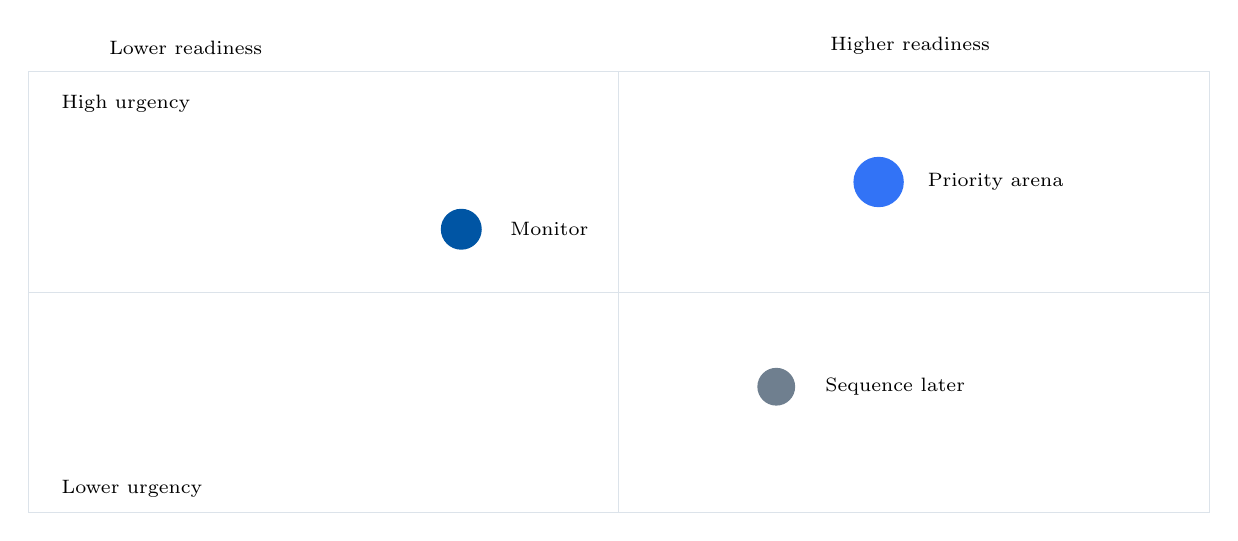
\begin{tikzpicture}[x=1mm,y=1mm]
\draw[BOLine] (0,0) rectangle (150,56);
\draw[BOLine] (75,0) -- (75,56); \draw[BOLine] (0,28) -- (150,28);
\node[anchor=west] at (3,52) {\scriptsize High urgency};
\node[anchor=west] at (3,3) {\scriptsize Lower urgency};
\node[anchor=south] at (20,57) {\scriptsize Lower readiness};
\node[anchor=south] at (112,57) {\scriptsize Higher readiness};
\fill[BOBright] (108,42) circle (3.2); \node[anchor=west] at (113,42) {\scriptsize Priority arena};
\fill[BOBlue] (55,36) circle (2.6); \node[anchor=west] at (60,36) {\scriptsize Monitor};
\fill[BOMuted] (95,16) circle (2.4); \node[anchor=west] at (100,16) {\scriptsize Sequence later};
\end{tikzpicture}
\end{center}

\clearpage
{\textcolor{BOBlue}{\scriptsize\bfseries MANAGEMENT IMPLICATIONS}}\par\vspace{-1pt}
{\Large\sffamily\bfseries\color{BONavy} Robotics Market Poised for Double-Digit Growth Driven by AI and Automation Demand}\par\vspace{4pt}
{\small The implication for executives is to translate the signal into a sequenced agenda: validate the facts, prioritize where the economics are strongest, and assign accountable owners for the next wave of decisions.}\par
\begin{tabularx}{\linewidth}{p{10mm}Y}
\textcolor{BOBlue}{\bfseries 1} & Prioritize management actions that change resource allocation. \\[5pt]
\textcolor{BOBlue}{\bfseries 2} & Validate the evidence base before committing capital. \\[5pt]
\textcolor{BOBlue}{\bfseries 3} & Sequence initiatives by materiality, feasibility and timing. \\[5pt]
\end{tabularx}
\vspace{6pt}

\vspace{6pt}{\textcolor{BOBlue}{\scriptsize\bfseries EXECUTION ROADMAP}}\par
\begin{center}

\begin{tikzpicture}[x=1mm,y=1mm]
\draw[very thick,BOBright] (10,18) -- (166,18);
\fill[BOBlue] (10,18) circle (2.2); \node[anchor=south,align=center,text width=34mm] at (10,22) {\scriptsize\textcolor{BOBlue}{\textbf{Now}}\\Confirm evidence};
\fill[BOBlue] (62,18) circle (2.2); \node[anchor=south,align=center,text width=34mm] at (62,22) {\scriptsize\textcolor{BOBlue}{\textbf{Next}}\\Prioritize moves};
\fill[BOBlue] (114,18) circle (2.2); \node[anchor=south,align=center,text width=34mm] at (114,22) {\scriptsize\textcolor{BOBlue}{\textbf{Then}}\\Commit resources};
\fill[BOBlue] (166,18) circle (2.2); \node[anchor=south,align=center,text width=34mm] at (166,22) {\scriptsize\textcolor{BOBlue}{\textbf{Scale}}\\Institutionalize};
\end{tikzpicture}
\end{center}

\clearpage
{\textcolor{BOBlue}{\scriptsize\bfseries CHAPTER 2}}\par\vspace{-1pt}
{\Large\sffamily\bfseries\color{BONavy} Industrial Robotics Dominates but Service Robotics Is the Fastest-Growing Segment}\par\vspace{4pt}
\begin{minipage}[t]{0.52\linewidth}
{\small Industrial Robotics Dominates but Service Robotics Is the Fastest-Growing Segment}\par
{\small The implication for executives is to translate the signal into a sequenced agenda: validate the facts, prioritize where the economics are strongest, and assign accountable owners for the next wave of decisions.}\par
\end{minipage}\hfill\begin{minipage}[t]{0.42\linewidth}

\includegraphics[width=74mm,height=54mm,keepaspectratio]{assets/image-2.png}
\end{minipage}
\vspace{5pt}
{\small The implication for executives is to translate the signal into a sequenced agenda: validate the facts, prioritize where the economics are strongest, and assign accountable owners for the next wave of decisions.}\par

\vspace{6pt}{\textcolor{BOBlue}{\scriptsize\bfseries DECISION LENS}}\par
\begin{tabularx}{\linewidth}{p{42mm}Y}
\textcolor{BOBlue}{\bfseries Question} & \textcolor{BOBlue}{\bfseries Why it matters} \\
Market direction & Separates structural change from temporary noise \\
Competitive response & Identifies where incumbents, challengers and customers may move next \\
Capital priority & Connects the argument to resource allocation and timing \\
\end{tabularx}

\clearpage
{\textcolor{BOBlue}{\scriptsize\bfseries EVIDENCE EXHIBIT}}\par\vspace{-1pt}
{\Large\sffamily\bfseries\color{BONavy} Industrial Robotics Dominates but Service Robotics Is the Fastest-Growing Segment}\par\vspace{4pt}

\includegraphics[width=170mm,height=88mm,keepaspectratio]{assets/chart-2.png}\vspace{5pt}
{\small The implication for executives is to translate the signal into a sequenced agenda: validate the facts, prioritize where the economics are strongest, and assign accountable owners for the next wave of decisions.}\par
{\small The exhibit should be read as directional evidence: it frames the relative magnitude, timing and management relevance of the issue rather than replacing diligence on the underlying source data.}\par

\vspace{6pt}{\textcolor{BOBlue}{\scriptsize\bfseries STRATEGIC POSITIONING MAP}}\par
\begin{center}
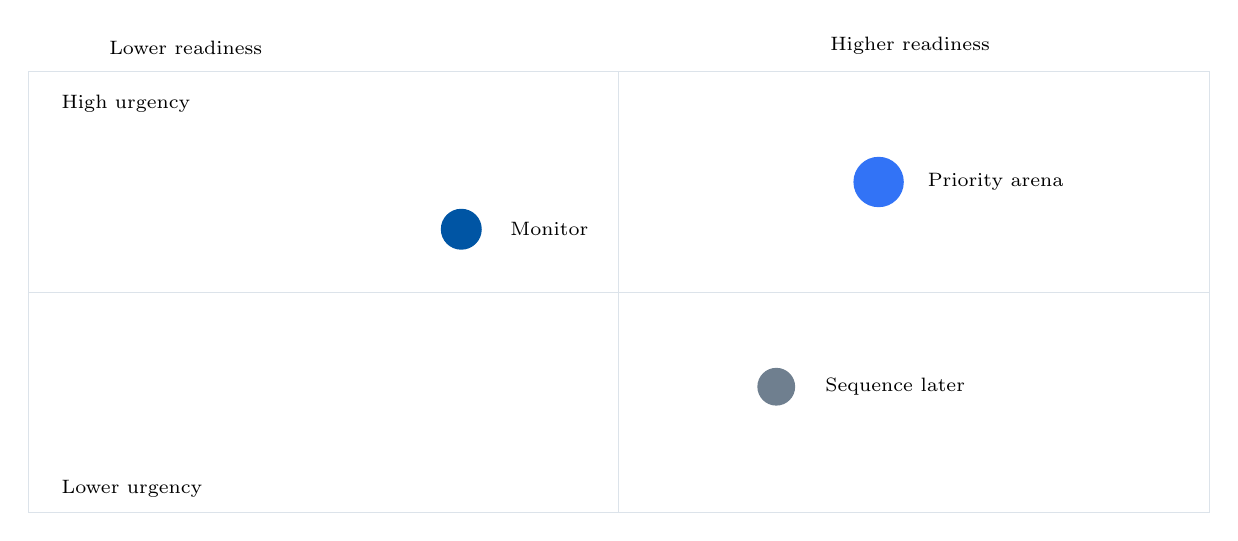
\begin{tikzpicture}[x=1mm,y=1mm]
\draw[BOLine] (0,0) rectangle (150,56);
\draw[BOLine] (75,0) -- (75,56); \draw[BOLine] (0,28) -- (150,28);
\node[anchor=west] at (3,52) {\scriptsize High urgency};
\node[anchor=west] at (3,3) {\scriptsize Lower urgency};
\node[anchor=south] at (20,57) {\scriptsize Lower readiness};
\node[anchor=south] at (112,57) {\scriptsize Higher readiness};
\fill[BOBright] (108,42) circle (3.2); \node[anchor=west] at (113,42) {\scriptsize Priority arena};
\fill[BOBlue] (55,36) circle (2.6); \node[anchor=west] at (60,36) {\scriptsize Monitor};
\fill[BOMuted] (95,16) circle (2.4); \node[anchor=west] at (100,16) {\scriptsize Sequence later};
\end{tikzpicture}
\end{center}

\clearpage
{\textcolor{BOBlue}{\scriptsize\bfseries MANAGEMENT IMPLICATIONS}}\par\vspace{-1pt}
{\Large\sffamily\bfseries\color{BONavy} Industrial Robotics Dominates but Service Robotics Is the Fastest-Growing Segment}\par\vspace{4pt}
{\small The implication for executives is to translate the signal into a sequenced agenda: validate the facts, prioritize where the economics are strongest, and assign accountable owners for the next wave of decisions.}\par
\begin{tabularx}{\linewidth}{p{10mm}Y}
\textcolor{BOBlue}{\bfseries 1} & Prioritize management actions that change resource allocation. \\[5pt]
\textcolor{BOBlue}{\bfseries 2} & Validate the evidence base before committing capital. \\[5pt]
\textcolor{BOBlue}{\bfseries 3} & Sequence initiatives by materiality, feasibility and timing. \\[5pt]
\end{tabularx}
\vspace{6pt}

\vspace{6pt}{\textcolor{BOBlue}{\scriptsize\bfseries EXECUTION ROADMAP}}\par
\begin{center}

\begin{tikzpicture}[x=1mm,y=1mm]
\draw[very thick,BOBright] (10,18) -- (166,18);
\fill[BOBlue] (10,18) circle (2.2); \node[anchor=south,align=center,text width=34mm] at (10,22) {\scriptsize\textcolor{BOBlue}{\textbf{Now}}\\Confirm evidence};
\fill[BOBlue] (62,18) circle (2.2); \node[anchor=south,align=center,text width=34mm] at (62,22) {\scriptsize\textcolor{BOBlue}{\textbf{Next}}\\Prioritize moves};
\fill[BOBlue] (114,18) circle (2.2); \node[anchor=south,align=center,text width=34mm] at (114,22) {\scriptsize\textcolor{BOBlue}{\textbf{Then}}\\Commit resources};
\fill[BOBlue] (166,18) circle (2.2); \node[anchor=south,align=center,text width=34mm] at (166,22) {\scriptsize\textcolor{BOBlue}{\textbf{Scale}}\\Institutionalize};
\end{tikzpicture}
\end{center}

\clearpage
{\textcolor{BOBlue}{\scriptsize\bfseries CHAPTER 3}}\par\vspace{-1pt}
{\Large\sffamily\bfseries\color{BONavy} Asia-Pacific Leads in Production and Adoption, with China as the Largest Market}\par\vspace{4pt}
\begin{minipage}[t]{0.52\linewidth}
{\small Asia-Pacific Leads in Production and Adoption, with China as the Largest Market}\par
{\small The implication for executives is to translate the signal into a sequenced agenda: validate the facts, prioritize where the economics are strongest, and assign accountable owners for the next wave of decisions.}\par
\end{minipage}\hfill\begin{minipage}[t]{0.42\linewidth}

\includegraphics[width=74mm,height=54mm,keepaspectratio]{assets/image-3.png}
\end{minipage}
\vspace{5pt}
{\small The implication for executives is to translate the signal into a sequenced agenda: validate the facts, prioritize where the economics are strongest, and assign accountable owners for the next wave of decisions.}\par

\vspace{6pt}{\textcolor{BOBlue}{\scriptsize\bfseries DECISION LENS}}\par
\begin{tabularx}{\linewidth}{p{42mm}Y}
\textcolor{BOBlue}{\bfseries Question} & \textcolor{BOBlue}{\bfseries Why it matters} \\
Market direction & Separates structural change from temporary noise \\
Competitive response & Identifies where incumbents, challengers and customers may move next \\
Capital priority & Connects the argument to resource allocation and timing \\
\end{tabularx}

\clearpage
{\textcolor{BOBlue}{\scriptsize\bfseries EVIDENCE EXHIBIT}}\par\vspace{-1pt}
{\Large\sffamily\bfseries\color{BONavy} Asia-Pacific Leads in Production and Adoption, with China as the Largest Market}\par\vspace{4pt}

\includegraphics[width=170mm,height=88mm,keepaspectratio]{assets/chart-3.png}\vspace{5pt}
{\small The implication for executives is to translate the signal into a sequenced agenda: validate the facts, prioritize where the economics are strongest, and assign accountable owners for the next wave of decisions.}\par
{\small The exhibit should be read as directional evidence: it frames the relative magnitude, timing and management relevance of the issue rather than replacing diligence on the underlying source data.}\par

\vspace{6pt}{\textcolor{BOBlue}{\scriptsize\bfseries STRATEGIC POSITIONING MAP}}\par
\begin{center}
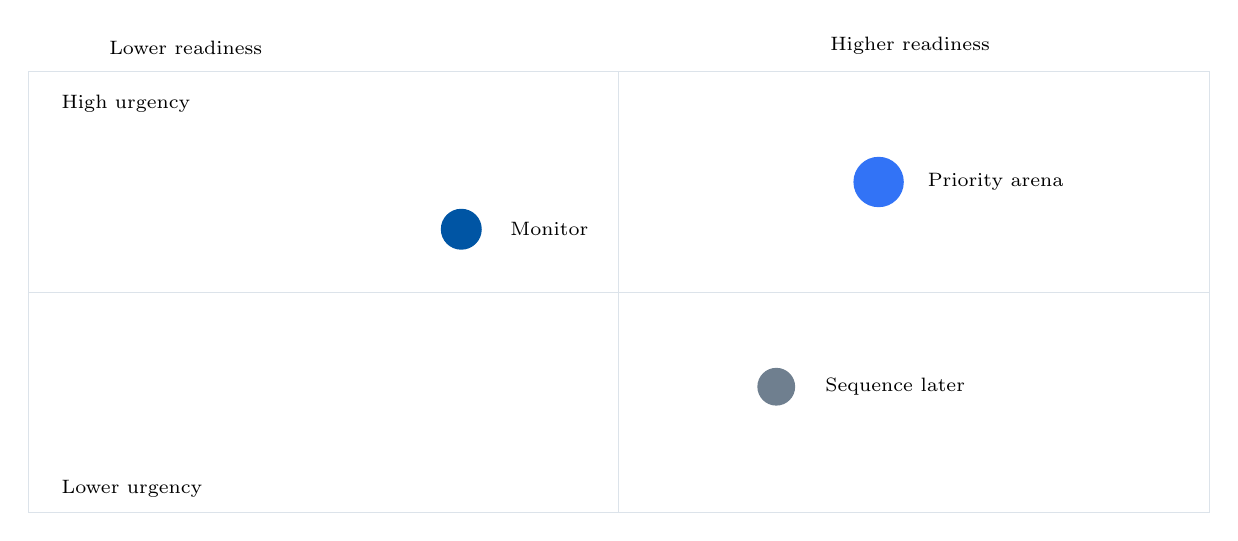
\begin{tikzpicture}[x=1mm,y=1mm]
\draw[BOLine] (0,0) rectangle (150,56);
\draw[BOLine] (75,0) -- (75,56); \draw[BOLine] (0,28) -- (150,28);
\node[anchor=west] at (3,52) {\scriptsize High urgency};
\node[anchor=west] at (3,3) {\scriptsize Lower urgency};
\node[anchor=south] at (20,57) {\scriptsize Lower readiness};
\node[anchor=south] at (112,57) {\scriptsize Higher readiness};
\fill[BOBright] (108,42) circle (3.2); \node[anchor=west] at (113,42) {\scriptsize Priority arena};
\fill[BOBlue] (55,36) circle (2.6); \node[anchor=west] at (60,36) {\scriptsize Monitor};
\fill[BOMuted] (95,16) circle (2.4); \node[anchor=west] at (100,16) {\scriptsize Sequence later};
\end{tikzpicture}
\end{center}

\clearpage
{\textcolor{BOBlue}{\scriptsize\bfseries MANAGEMENT IMPLICATIONS}}\par\vspace{-1pt}
{\Large\sffamily\bfseries\color{BONavy} Asia-Pacific Leads in Production and Adoption, with China as the Largest Market}\par\vspace{4pt}
{\small The implication for executives is to translate the signal into a sequenced agenda: validate the facts, prioritize where the economics are strongest, and assign accountable owners for the next wave of decisions.}\par
\begin{tabularx}{\linewidth}{p{10mm}Y}
\textcolor{BOBlue}{\bfseries 1} & Prioritize management actions that change resource allocation. \\[5pt]
\textcolor{BOBlue}{\bfseries 2} & Validate the evidence base before committing capital. \\[5pt]
\textcolor{BOBlue}{\bfseries 3} & Sequence initiatives by materiality, feasibility and timing. \\[5pt]
\end{tabularx}
\vspace{6pt}

\vspace{6pt}{\textcolor{BOBlue}{\scriptsize\bfseries EXECUTION ROADMAP}}\par
\begin{center}

\begin{tikzpicture}[x=1mm,y=1mm]
\draw[very thick,BOBright] (10,18) -- (166,18);
\fill[BOBlue] (10,18) circle (2.2); \node[anchor=south,align=center,text width=34mm] at (10,22) {\scriptsize\textcolor{BOBlue}{\textbf{Now}}\\Confirm evidence};
\fill[BOBlue] (62,18) circle (2.2); \node[anchor=south,align=center,text width=34mm] at (62,22) {\scriptsize\textcolor{BOBlue}{\textbf{Next}}\\Prioritize moves};
\fill[BOBlue] (114,18) circle (2.2); \node[anchor=south,align=center,text width=34mm] at (114,22) {\scriptsize\textcolor{BOBlue}{\textbf{Then}}\\Commit resources};
\fill[BOBlue] (166,18) circle (2.2); \node[anchor=south,align=center,text width=34mm] at (166,22) {\scriptsize\textcolor{BOBlue}{\textbf{Scale}}\\Institutionalize};
\end{tikzpicture}
\end{center}

\clearpage
{\textcolor{BOBlue}{\scriptsize\bfseries CHAPTER 4}}\par\vspace{-1pt}
{\Large\sffamily\bfseries\color{BONavy} Incumbents Hold Strong Positions but Face Disruption from Agile Startups and Tech Giants}\par\vspace{4pt}
\begin{minipage}[t]{0.52\linewidth}
{\small Incumbents Hold Strong Positions but Face Disruption from Agile Startups and Tech Giants}\par
{\small The implication for executives is to translate the signal into a sequenced agenda: validate the facts, prioritize where the economics are strongest, and assign accountable owners for the next wave of decisions.}\par
\end{minipage}\hfill\begin{minipage}[t]{0.42\linewidth}

\includegraphics[width=74mm,height=54mm,keepaspectratio]{assets/image-4.png}
\end{minipage}
\vspace{5pt}
{\small The implication for executives is to translate the signal into a sequenced agenda: validate the facts, prioritize where the economics are strongest, and assign accountable owners for the next wave of decisions.}\par

\vspace{6pt}{\textcolor{BOBlue}{\scriptsize\bfseries DECISION LENS}}\par
\begin{tabularx}{\linewidth}{p{42mm}Y}
\textcolor{BOBlue}{\bfseries Question} & \textcolor{BOBlue}{\bfseries Why it matters} \\
Market direction & Separates structural change from temporary noise \\
Competitive response & Identifies where incumbents, challengers and customers may move next \\
Capital priority & Connects the argument to resource allocation and timing \\
\end{tabularx}

\clearpage
{\textcolor{BOBlue}{\scriptsize\bfseries EVIDENCE EXHIBIT}}\par\vspace{-1pt}
{\Large\sffamily\bfseries\color{BONavy} Incumbents Hold Strong Positions but Face Disruption from Agile Startups and Tech Giants}\par\vspace{4pt}

\includegraphics[width=170mm,height=88mm,keepaspectratio]{assets/chart-4.png}\vspace{5pt}
{\small The implication for executives is to translate the signal into a sequenced agenda: validate the facts, prioritize where the economics are strongest, and assign accountable owners for the next wave of decisions.}\par
{\small The exhibit should be read as directional evidence: it frames the relative magnitude, timing and management relevance of the issue rather than replacing diligence on the underlying source data.}\par

\vspace{6pt}{\textcolor{BOBlue}{\scriptsize\bfseries STRATEGIC POSITIONING MAP}}\par
\begin{center}
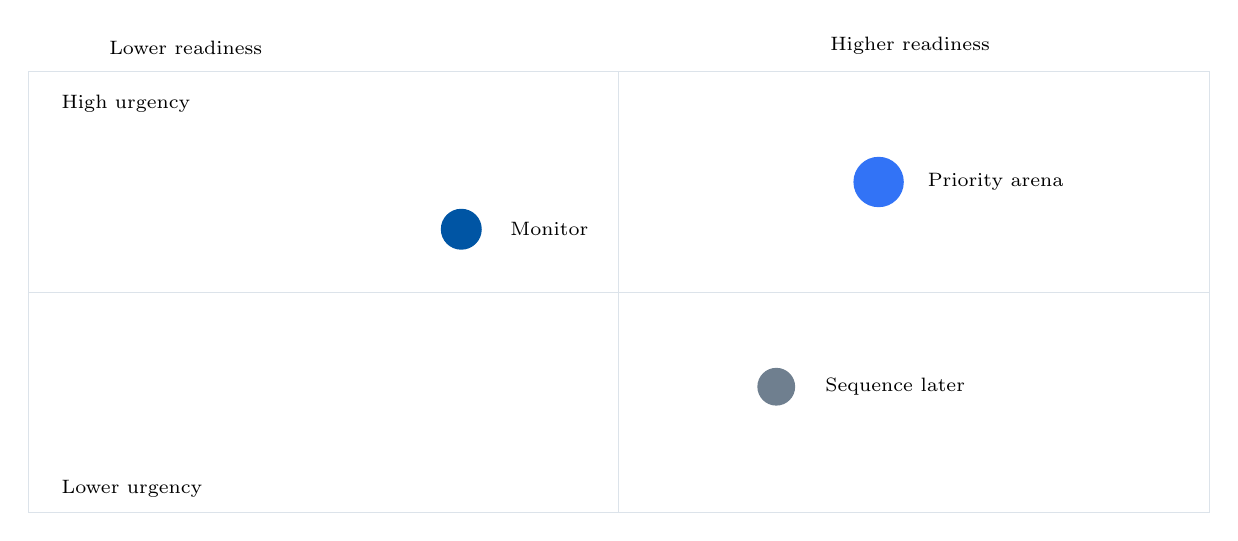
\begin{tikzpicture}[x=1mm,y=1mm]
\draw[BOLine] (0,0) rectangle (150,56);
\draw[BOLine] (75,0) -- (75,56); \draw[BOLine] (0,28) -- (150,28);
\node[anchor=west] at (3,52) {\scriptsize High urgency};
\node[anchor=west] at (3,3) {\scriptsize Lower urgency};
\node[anchor=south] at (20,57) {\scriptsize Lower readiness};
\node[anchor=south] at (112,57) {\scriptsize Higher readiness};
\fill[BOBright] (108,42) circle (3.2); \node[anchor=west] at (113,42) {\scriptsize Priority arena};
\fill[BOBlue] (55,36) circle (2.6); \node[anchor=west] at (60,36) {\scriptsize Monitor};
\fill[BOMuted] (95,16) circle (2.4); \node[anchor=west] at (100,16) {\scriptsize Sequence later};
\end{tikzpicture}
\end{center}

\clearpage
{\textcolor{BOBlue}{\scriptsize\bfseries MANAGEMENT IMPLICATIONS}}\par\vspace{-1pt}
{\Large\sffamily\bfseries\color{BONavy} Incumbents Hold Strong Positions but Face Disruption from Agile Startups and Tech Giants}\par\vspace{4pt}
{\small The implication for executives is to translate the signal into a sequenced agenda: validate the facts, prioritize where the economics are strongest, and assign accountable owners for the next wave of decisions.}\par
\begin{tabularx}{\linewidth}{p{10mm}Y}
\textcolor{BOBlue}{\bfseries 1} & Prioritize management actions that change resource allocation. \\[5pt]
\textcolor{BOBlue}{\bfseries 2} & Validate the evidence base before committing capital. \\[5pt]
\textcolor{BOBlue}{\bfseries 3} & Sequence initiatives by materiality, feasibility and timing. \\[5pt]
\end{tabularx}
\vspace{6pt}

\vspace{6pt}{\textcolor{BOBlue}{\scriptsize\bfseries EXECUTION ROADMAP}}\par
\begin{center}

\begin{tikzpicture}[x=1mm,y=1mm]
\draw[very thick,BOBright] (10,18) -- (166,18);
\fill[BOBlue] (10,18) circle (2.2); \node[anchor=south,align=center,text width=34mm] at (10,22) {\scriptsize\textcolor{BOBlue}{\textbf{Now}}\\Confirm evidence};
\fill[BOBlue] (62,18) circle (2.2); \node[anchor=south,align=center,text width=34mm] at (62,22) {\scriptsize\textcolor{BOBlue}{\textbf{Next}}\\Prioritize moves};
\fill[BOBlue] (114,18) circle (2.2); \node[anchor=south,align=center,text width=34mm] at (114,22) {\scriptsize\textcolor{BOBlue}{\textbf{Then}}\\Commit resources};
\fill[BOBlue] (166,18) circle (2.2); \node[anchor=south,align=center,text width=34mm] at (166,22) {\scriptsize\textcolor{BOBlue}{\textbf{Scale}}\\Institutionalize};
\end{tikzpicture}
\end{center}

\clearpage
{\textcolor{BOBlue}{\scriptsize\bfseries CHAPTER 5}}\par\vspace{-1pt}
{\Large\sffamily\bfseries\color{BONavy} Collaborative Robots and Autonomous Mobile Robots Are Reshaping Factory and Warehouse Operations}\par\vspace{4pt}
\begin{minipage}[t]{0.52\linewidth}
{\small Collaborative Robots and Autonomous Mobile Robots Are Reshaping Factory and Warehouse Operations}\par
{\small The implication for executives is to translate the signal into a sequenced agenda: validate the facts, prioritize where the economics are strongest, and assign accountable owners for the next wave of decisions.}\par
\end{minipage}\hfill\begin{minipage}[t]{0.42\linewidth}

\includegraphics[width=74mm,height=54mm,keepaspectratio]{assets/image-5.png}
\end{minipage}
\vspace{5pt}
{\small The implication for executives is to translate the signal into a sequenced agenda: validate the facts, prioritize where the economics are strongest, and assign accountable owners for the next wave of decisions.}\par

\vspace{6pt}{\textcolor{BOBlue}{\scriptsize\bfseries DECISION LENS}}\par
\begin{tabularx}{\linewidth}{p{42mm}Y}
\textcolor{BOBlue}{\bfseries Question} & \textcolor{BOBlue}{\bfseries Why it matters} \\
Market direction & Separates structural change from temporary noise \\
Competitive response & Identifies where incumbents, challengers and customers may move next \\
Capital priority & Connects the argument to resource allocation and timing \\
\end{tabularx}

\clearpage
{\textcolor{BOBlue}{\scriptsize\bfseries EVIDENCE EXHIBIT}}\par\vspace{-1pt}
{\Large\sffamily\bfseries\color{BONavy} Collaborative Robots and Autonomous Mobile Robots Are Reshaping Factory and Warehouse Operations}\par\vspace{4pt}

\includegraphics[width=170mm,height=88mm,keepaspectratio]{assets/chart-5.png}\vspace{5pt}
{\small The implication for executives is to translate the signal into a sequenced agenda: validate the facts, prioritize where the economics are strongest, and assign accountable owners for the next wave of decisions.}\par
{\small The exhibit should be read as directional evidence: it frames the relative magnitude, timing and management relevance of the issue rather than replacing diligence on the underlying source data.}\par

\vspace{6pt}{\textcolor{BOBlue}{\scriptsize\bfseries STRATEGIC POSITIONING MAP}}\par
\begin{center}
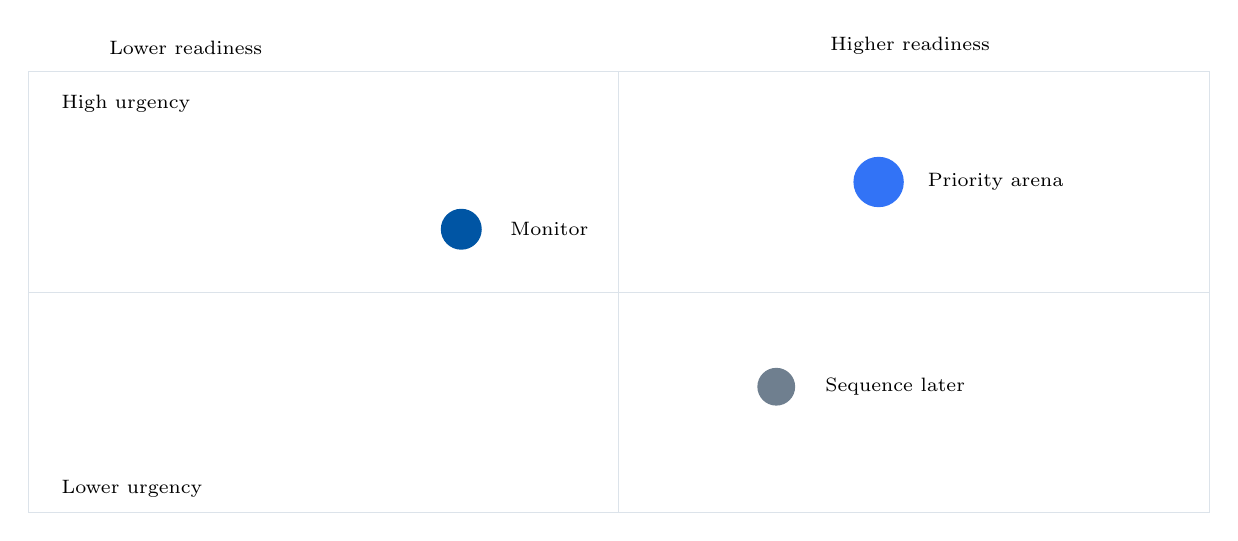
\begin{tikzpicture}[x=1mm,y=1mm]
\draw[BOLine] (0,0) rectangle (150,56);
\draw[BOLine] (75,0) -- (75,56); \draw[BOLine] (0,28) -- (150,28);
\node[anchor=west] at (3,52) {\scriptsize High urgency};
\node[anchor=west] at (3,3) {\scriptsize Lower urgency};
\node[anchor=south] at (20,57) {\scriptsize Lower readiness};
\node[anchor=south] at (112,57) {\scriptsize Higher readiness};
\fill[BOBright] (108,42) circle (3.2); \node[anchor=west] at (113,42) {\scriptsize Priority arena};
\fill[BOBlue] (55,36) circle (2.6); \node[anchor=west] at (60,36) {\scriptsize Monitor};
\fill[BOMuted] (95,16) circle (2.4); \node[anchor=west] at (100,16) {\scriptsize Sequence later};
\end{tikzpicture}
\end{center}

\clearpage
{\textcolor{BOBlue}{\scriptsize\bfseries MANAGEMENT IMPLICATIONS}}\par\vspace{-1pt}
{\Large\sffamily\bfseries\color{BONavy} Collaborative Robots and Autonomous Mobile Robots Are Reshaping Factory and Warehouse Operations}\par\vspace{4pt}
{\small The implication for executives is to translate the signal into a sequenced agenda: validate the facts, prioritize where the economics are strongest, and assign accountable owners for the next wave of decisions.}\par
\begin{tabularx}{\linewidth}{p{10mm}Y}
\textcolor{BOBlue}{\bfseries 1} & Prioritize management actions that change resource allocation. \\[5pt]
\textcolor{BOBlue}{\bfseries 2} & Validate the evidence base before committing capital. \\[5pt]
\textcolor{BOBlue}{\bfseries 3} & Sequence initiatives by materiality, feasibility and timing. \\[5pt]
\end{tabularx}
\vspace{6pt}

\vspace{6pt}{\textcolor{BOBlue}{\scriptsize\bfseries EXECUTION ROADMAP}}\par
\begin{center}

\begin{tikzpicture}[x=1mm,y=1mm]
\draw[very thick,BOBright] (10,18) -- (166,18);
\fill[BOBlue] (10,18) circle (2.2); \node[anchor=south,align=center,text width=34mm] at (10,22) {\scriptsize\textcolor{BOBlue}{\textbf{Now}}\\Confirm evidence};
\fill[BOBlue] (62,18) circle (2.2); \node[anchor=south,align=center,text width=34mm] at (62,22) {\scriptsize\textcolor{BOBlue}{\textbf{Next}}\\Prioritize moves};
\fill[BOBlue] (114,18) circle (2.2); \node[anchor=south,align=center,text width=34mm] at (114,22) {\scriptsize\textcolor{BOBlue}{\textbf{Then}}\\Commit resources};
\fill[BOBlue] (166,18) circle (2.2); \node[anchor=south,align=center,text width=34mm] at (166,22) {\scriptsize\textcolor{BOBlue}{\textbf{Scale}}\\Institutionalize};
\end{tikzpicture}
\end{center}

\clearpage
{\textcolor{BOBlue}{\scriptsize\bfseries CHAPTER 6}}\par\vspace{-1pt}
{\Large\sffamily\bfseries\color{BONavy} Robot-as-a-Service Lowers Entry Barriers and Accelerates Adoption Among SMEs}\par\vspace{4pt}
\begin{minipage}[t]{0.52\linewidth}
{\small Robot-as-a-Service Lowers Entry Barriers and Accelerates Adoption Among SMEs}\par
{\small The implication for executives is to translate the signal into a sequenced agenda: validate the facts, prioritize where the economics are strongest, and assign accountable owners for the next wave of decisions.}\par
\end{minipage}\hfill\begin{minipage}[t]{0.42\linewidth}

\includegraphics[width=74mm,height=54mm,keepaspectratio]{assets/image-6.png}
\end{minipage}
\vspace{5pt}
{\small The implication for executives is to translate the signal into a sequenced agenda: validate the facts, prioritize where the economics are strongest, and assign accountable owners for the next wave of decisions.}\par

\vspace{6pt}{\textcolor{BOBlue}{\scriptsize\bfseries DECISION LENS}}\par
\begin{tabularx}{\linewidth}{p{42mm}Y}
\textcolor{BOBlue}{\bfseries Question} & \textcolor{BOBlue}{\bfseries Why it matters} \\
Market direction & Separates structural change from temporary noise \\
Competitive response & Identifies where incumbents, challengers and customers may move next \\
Capital priority & Connects the argument to resource allocation and timing \\
\end{tabularx}

\clearpage
{\textcolor{BOBlue}{\scriptsize\bfseries EVIDENCE EXHIBIT}}\par\vspace{-1pt}
{\Large\sffamily\bfseries\color{BONavy} Robot-as-a-Service Lowers Entry Barriers and Accelerates Adoption Among SMEs}\par\vspace{4pt}

\includegraphics[width=170mm,height=88mm,keepaspectratio]{assets/chart-6.png}\vspace{5pt}
{\small The implication for executives is to translate the signal into a sequenced agenda: validate the facts, prioritize where the economics are strongest, and assign accountable owners for the next wave of decisions.}\par
{\small The exhibit should be read as directional evidence: it frames the relative magnitude, timing and management relevance of the issue rather than replacing diligence on the underlying source data.}\par

\vspace{6pt}{\textcolor{BOBlue}{\scriptsize\bfseries STRATEGIC POSITIONING MAP}}\par
\begin{center}
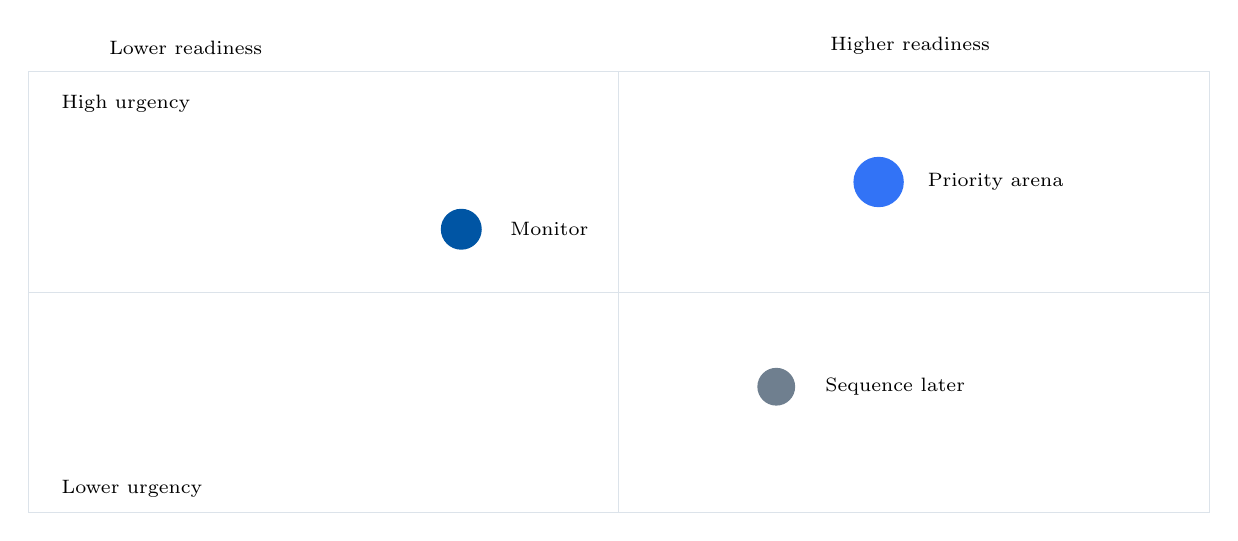
\begin{tikzpicture}[x=1mm,y=1mm]
\draw[BOLine] (0,0) rectangle (150,56);
\draw[BOLine] (75,0) -- (75,56); \draw[BOLine] (0,28) -- (150,28);
\node[anchor=west] at (3,52) {\scriptsize High urgency};
\node[anchor=west] at (3,3) {\scriptsize Lower urgency};
\node[anchor=south] at (20,57) {\scriptsize Lower readiness};
\node[anchor=south] at (112,57) {\scriptsize Higher readiness};
\fill[BOBright] (108,42) circle (3.2); \node[anchor=west] at (113,42) {\scriptsize Priority arena};
\fill[BOBlue] (55,36) circle (2.6); \node[anchor=west] at (60,36) {\scriptsize Monitor};
\fill[BOMuted] (95,16) circle (2.4); \node[anchor=west] at (100,16) {\scriptsize Sequence later};
\end{tikzpicture}
\end{center}

\clearpage
{\textcolor{BOBlue}{\scriptsize\bfseries MANAGEMENT IMPLICATIONS}}\par\vspace{-1pt}
{\Large\sffamily\bfseries\color{BONavy} Robot-as-a-Service Lowers Entry Barriers and Accelerates Adoption Among SMEs}\par\vspace{4pt}
{\small The implication for executives is to translate the signal into a sequenced agenda: validate the facts, prioritize where the economics are strongest, and assign accountable owners for the next wave of decisions.}\par
\begin{tabularx}{\linewidth}{p{10mm}Y}
\textcolor{BOBlue}{\bfseries 1} & Prioritize management actions that change resource allocation. \\[5pt]
\textcolor{BOBlue}{\bfseries 2} & Validate the evidence base before committing capital. \\[5pt]
\textcolor{BOBlue}{\bfseries 3} & Sequence initiatives by materiality, feasibility and timing. \\[5pt]
\end{tabularx}
\vspace{6pt}

\vspace{6pt}{\textcolor{BOBlue}{\scriptsize\bfseries EXECUTION ROADMAP}}\par
\begin{center}

\begin{tikzpicture}[x=1mm,y=1mm]
\draw[very thick,BOBright] (10,18) -- (166,18);
\fill[BOBlue] (10,18) circle (2.2); \node[anchor=south,align=center,text width=34mm] at (10,22) {\scriptsize\textcolor{BOBlue}{\textbf{Now}}\\Confirm evidence};
\fill[BOBlue] (62,18) circle (2.2); \node[anchor=south,align=center,text width=34mm] at (62,22) {\scriptsize\textcolor{BOBlue}{\textbf{Next}}\\Prioritize moves};
\fill[BOBlue] (114,18) circle (2.2); \node[anchor=south,align=center,text width=34mm] at (114,22) {\scriptsize\textcolor{BOBlue}{\textbf{Then}}\\Commit resources};
\fill[BOBlue] (166,18) circle (2.2); \node[anchor=south,align=center,text width=34mm] at (166,22) {\scriptsize\textcolor{BOBlue}{\textbf{Scale}}\\Institutionalize};
\end{tikzpicture}
\end{center}

\clearpage
{\textcolor{BOBlue}{\scriptsize\bfseries CHAPTER 7}}\par\vspace{-1pt}
{\Large\sffamily\bfseries\color{BONavy} Regulatory Frameworks Are Evolving but Remain Fragmented Across Regions}\par\vspace{4pt}
\begin{minipage}[t]{0.52\linewidth}
{\small Regulatory Frameworks Are Evolving but Remain Fragmented Across Regions}\par
{\small The implication for executives is to translate the signal into a sequenced agenda: validate the facts, prioritize where the economics are strongest, and assign accountable owners for the next wave of decisions.}\par
\end{minipage}\hfill\begin{minipage}[t]{0.42\linewidth}

\includegraphics[width=74mm,height=54mm,keepaspectratio]{assets/image-7.png}
\end{minipage}
\vspace{5pt}
{\small The implication for executives is to translate the signal into a sequenced agenda: validate the facts, prioritize where the economics are strongest, and assign accountable owners for the next wave of decisions.}\par

\vspace{6pt}{\textcolor{BOBlue}{\scriptsize\bfseries DECISION LENS}}\par
\begin{tabularx}{\linewidth}{p{42mm}Y}
\textcolor{BOBlue}{\bfseries Question} & \textcolor{BOBlue}{\bfseries Why it matters} \\
Market direction & Separates structural change from temporary noise \\
Competitive response & Identifies where incumbents, challengers and customers may move next \\
Capital priority & Connects the argument to resource allocation and timing \\
\end{tabularx}

\clearpage
{\textcolor{BOBlue}{\scriptsize\bfseries EVIDENCE EXHIBIT}}\par\vspace{-1pt}
{\Large\sffamily\bfseries\color{BONavy} Regulatory Frameworks Are Evolving but Remain Fragmented Across Regions}\par\vspace{4pt}

\includegraphics[width=170mm,height=88mm,keepaspectratio]{assets/chart-7.png}\vspace{5pt}
{\small The implication for executives is to translate the signal into a sequenced agenda: validate the facts, prioritize where the economics are strongest, and assign accountable owners for the next wave of decisions.}\par
{\small The exhibit should be read as directional evidence: it frames the relative magnitude, timing and management relevance of the issue rather than replacing diligence on the underlying source data.}\par

\vspace{6pt}{\textcolor{BOBlue}{\scriptsize\bfseries STRATEGIC POSITIONING MAP}}\par
\begin{center}
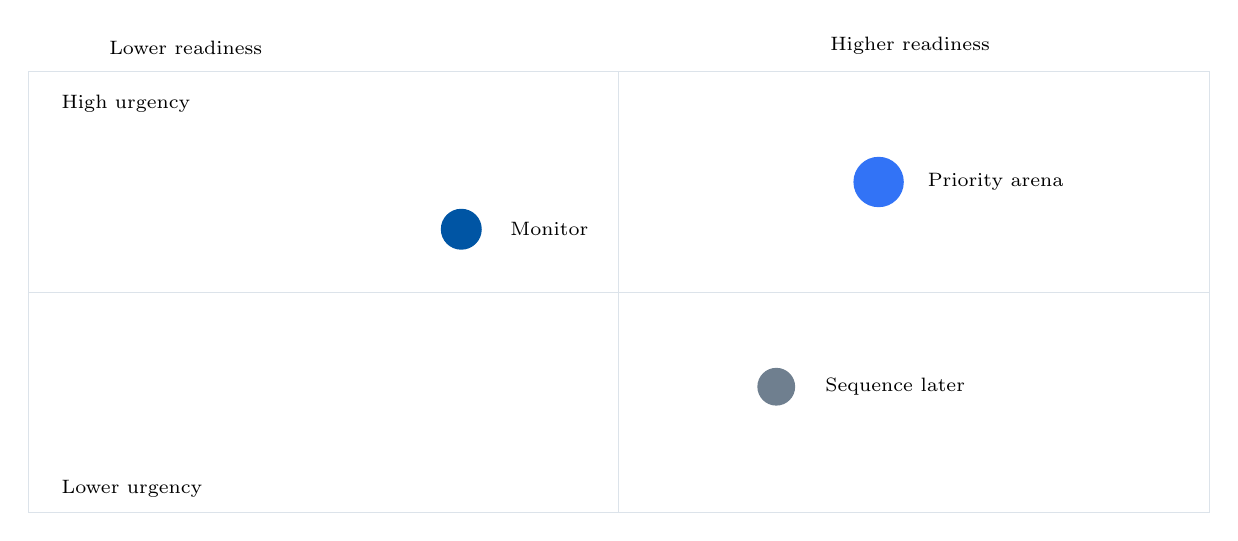
\begin{tikzpicture}[x=1mm,y=1mm]
\draw[BOLine] (0,0) rectangle (150,56);
\draw[BOLine] (75,0) -- (75,56); \draw[BOLine] (0,28) -- (150,28);
\node[anchor=west] at (3,52) {\scriptsize High urgency};
\node[anchor=west] at (3,3) {\scriptsize Lower urgency};
\node[anchor=south] at (20,57) {\scriptsize Lower readiness};
\node[anchor=south] at (112,57) {\scriptsize Higher readiness};
\fill[BOBright] (108,42) circle (3.2); \node[anchor=west] at (113,42) {\scriptsize Priority arena};
\fill[BOBlue] (55,36) circle (2.6); \node[anchor=west] at (60,36) {\scriptsize Monitor};
\fill[BOMuted] (95,16) circle (2.4); \node[anchor=west] at (100,16) {\scriptsize Sequence later};
\end{tikzpicture}
\end{center}

\clearpage
{\textcolor{BOBlue}{\scriptsize\bfseries MANAGEMENT IMPLICATIONS}}\par\vspace{-1pt}
{\Large\sffamily\bfseries\color{BONavy} Regulatory Frameworks Are Evolving but Remain Fragmented Across Regions}\par\vspace{4pt}
{\small The implication for executives is to translate the signal into a sequenced agenda: validate the facts, prioritize where the economics are strongest, and assign accountable owners for the next wave of decisions.}\par
\begin{tabularx}{\linewidth}{p{10mm}Y}
\textcolor{BOBlue}{\bfseries 1} & Prioritize management actions that change resource allocation. \\[5pt]
\textcolor{BOBlue}{\bfseries 2} & Validate the evidence base before committing capital. \\[5pt]
\textcolor{BOBlue}{\bfseries 3} & Sequence initiatives by materiality, feasibility and timing. \\[5pt]
\end{tabularx}
\vspace{6pt}

\vspace{6pt}{\textcolor{BOBlue}{\scriptsize\bfseries EXECUTION ROADMAP}}\par
\begin{center}

\begin{tikzpicture}[x=1mm,y=1mm]
\draw[very thick,BOBright] (10,18) -- (166,18);
\fill[BOBlue] (10,18) circle (2.2); \node[anchor=south,align=center,text width=34mm] at (10,22) {\scriptsize\textcolor{BOBlue}{\textbf{Now}}\\Confirm evidence};
\fill[BOBlue] (62,18) circle (2.2); \node[anchor=south,align=center,text width=34mm] at (62,22) {\scriptsize\textcolor{BOBlue}{\textbf{Next}}\\Prioritize moves};
\fill[BOBlue] (114,18) circle (2.2); \node[anchor=south,align=center,text width=34mm] at (114,22) {\scriptsize\textcolor{BOBlue}{\textbf{Then}}\\Commit resources};
\fill[BOBlue] (166,18) circle (2.2); \node[anchor=south,align=center,text width=34mm] at (166,22) {\scriptsize\textcolor{BOBlue}{\textbf{Scale}}\\Institutionalize};
\end{tikzpicture}
\end{center}

\clearpage
{\textcolor{BOBlue}{\scriptsize\bfseries CHAPTER 8}}\par\vspace{-1pt}
{\Large\sffamily\bfseries\color{BONavy} Ethical and Social Concerns Require Proactive Workforce Transition Strategies}\par\vspace{4pt}
\begin{minipage}[t]{0.52\linewidth}
{\small Ethical and Social Concerns Require Proactive Workforce Transition Strategies}\par
{\small The implication for executives is to translate the signal into a sequenced agenda: validate the facts, prioritize where the economics are strongest, and assign accountable owners for the next wave of decisions.}\par
\end{minipage}\hfill\begin{minipage}[t]{0.42\linewidth}

\includegraphics[width=74mm,height=54mm,keepaspectratio]{assets/image-8.png}
\end{minipage}
\vspace{5pt}
{\small The implication for executives is to translate the signal into a sequenced agenda: validate the facts, prioritize where the economics are strongest, and assign accountable owners for the next wave of decisions.}\par

\vspace{6pt}{\textcolor{BOBlue}{\scriptsize\bfseries DECISION LENS}}\par
\begin{tabularx}{\linewidth}{p{42mm}Y}
\textcolor{BOBlue}{\bfseries Question} & \textcolor{BOBlue}{\bfseries Why it matters} \\
Market direction & Separates structural change from temporary noise \\
Competitive response & Identifies where incumbents, challengers and customers may move next \\
Capital priority & Connects the argument to resource allocation and timing \\
\end{tabularx}

\clearpage
{\textcolor{BOBlue}{\scriptsize\bfseries EVIDENCE EXHIBIT}}\par\vspace{-1pt}
{\Large\sffamily\bfseries\color{BONavy} Ethical and Social Concerns Require Proactive Workforce Transition Strategies}\par\vspace{4pt}

\includegraphics[width=170mm,height=88mm,keepaspectratio]{assets/chart-2.png}\vspace{5pt}
{\small The implication for executives is to translate the signal into a sequenced agenda: validate the facts, prioritize where the economics are strongest, and assign accountable owners for the next wave of decisions.}\par
{\small The exhibit should be read as directional evidence: it frames the relative magnitude, timing and management relevance of the issue rather than replacing diligence on the underlying source data.}\par

\vspace{6pt}{\textcolor{BOBlue}{\scriptsize\bfseries STRATEGIC POSITIONING MAP}}\par
\begin{center}
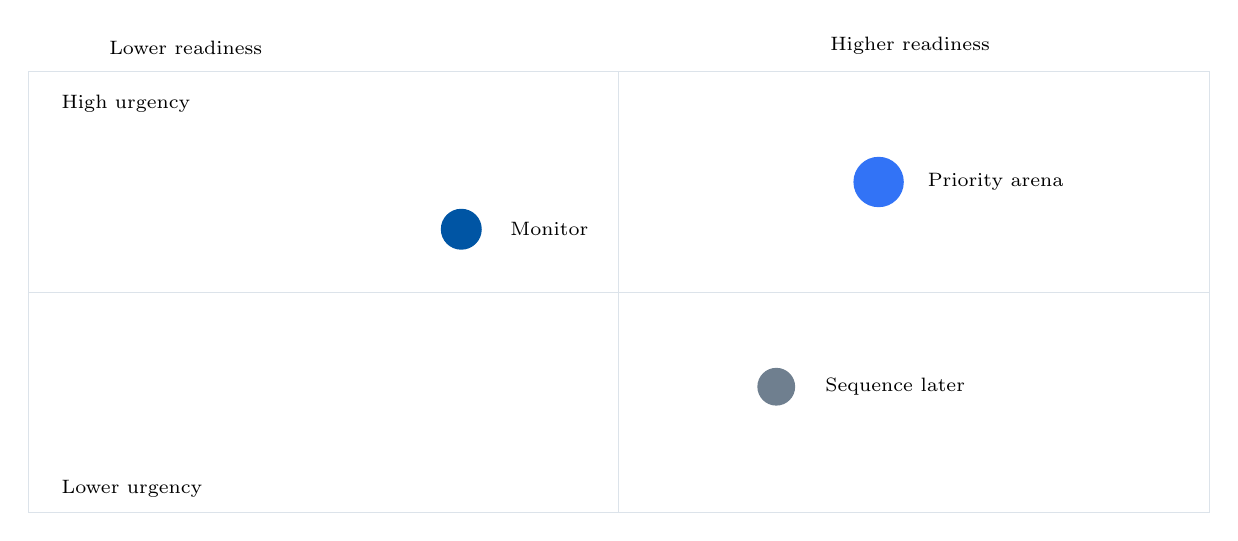
\begin{tikzpicture}[x=1mm,y=1mm]
\draw[BOLine] (0,0) rectangle (150,56);
\draw[BOLine] (75,0) -- (75,56); \draw[BOLine] (0,28) -- (150,28);
\node[anchor=west] at (3,52) {\scriptsize High urgency};
\node[anchor=west] at (3,3) {\scriptsize Lower urgency};
\node[anchor=south] at (20,57) {\scriptsize Lower readiness};
\node[anchor=south] at (112,57) {\scriptsize Higher readiness};
\fill[BOBright] (108,42) circle (3.2); \node[anchor=west] at (113,42) {\scriptsize Priority arena};
\fill[BOBlue] (55,36) circle (2.6); \node[anchor=west] at (60,36) {\scriptsize Monitor};
\fill[BOMuted] (95,16) circle (2.4); \node[anchor=west] at (100,16) {\scriptsize Sequence later};
\end{tikzpicture}
\end{center}

\clearpage
{\textcolor{BOBlue}{\scriptsize\bfseries MANAGEMENT IMPLICATIONS}}\par\vspace{-1pt}
{\Large\sffamily\bfseries\color{BONavy} Ethical and Social Concerns Require Proactive Workforce Transition Strategies}\par\vspace{4pt}
{\small The implication for executives is to translate the signal into a sequenced agenda: validate the facts, prioritize where the economics are strongest, and assign accountable owners for the next wave of decisions.}\par
\begin{tabularx}{\linewidth}{p{10mm}Y}
\textcolor{BOBlue}{\bfseries 1} & Prioritize management actions that change resource allocation. \\[5pt]
\textcolor{BOBlue}{\bfseries 2} & Validate the evidence base before committing capital. \\[5pt]
\textcolor{BOBlue}{\bfseries 3} & Sequence initiatives by materiality, feasibility and timing. \\[5pt]
\end{tabularx}
\vspace{6pt}

\vspace{6pt}{\textcolor{BOBlue}{\scriptsize\bfseries EXECUTION ROADMAP}}\par
\begin{center}

\begin{tikzpicture}[x=1mm,y=1mm]
\draw[very thick,BOBright] (10,18) -- (166,18);
\fill[BOBlue] (10,18) circle (2.2); \node[anchor=south,align=center,text width=34mm] at (10,22) {\scriptsize\textcolor{BOBlue}{\textbf{Now}}\\Confirm evidence};
\fill[BOBlue] (62,18) circle (2.2); \node[anchor=south,align=center,text width=34mm] at (62,22) {\scriptsize\textcolor{BOBlue}{\textbf{Next}}\\Prioritize moves};
\fill[BOBlue] (114,18) circle (2.2); \node[anchor=south,align=center,text width=34mm] at (114,22) {\scriptsize\textcolor{BOBlue}{\textbf{Then}}\\Commit resources};
\fill[BOBlue] (166,18) circle (2.2); \node[anchor=south,align=center,text width=34mm] at (166,22) {\scriptsize\textcolor{BOBlue}{\textbf{Scale}}\\Institutionalize};
\end{tikzpicture}
\end{center}

\clearpage
{\textcolor{BOBlue}{\scriptsize\bfseries CHAPTER 9}}\par\vspace{-1pt}
{\Large\sffamily\bfseries\color{BONavy} Healthcare and Logistics Offer the Highest Near-Term Growth Opportunities}\par\vspace{4pt}
\begin{minipage}[t]{0.52\linewidth}
{\small Healthcare and Logistics Offer the Highest Near-Term Growth Opportunities}\par
{\small The implication for executives is to translate the signal into a sequenced agenda: validate the facts, prioritize where the economics are strongest, and assign accountable owners for the next wave of decisions.}\par
\end{minipage}\hfill\begin{minipage}[t]{0.42\linewidth}

\includegraphics[width=74mm,height=54mm,keepaspectratio]{assets/image-9.png}
\end{minipage}
\vspace{5pt}
{\small The implication for executives is to translate the signal into a sequenced agenda: validate the facts, prioritize where the economics are strongest, and assign accountable owners for the next wave of decisions.}\par

\vspace{6pt}{\textcolor{BOBlue}{\scriptsize\bfseries DECISION LENS}}\par
\begin{tabularx}{\linewidth}{p{42mm}Y}
\textcolor{BOBlue}{\bfseries Question} & \textcolor{BOBlue}{\bfseries Why it matters} \\
Market direction & Separates structural change from temporary noise \\
Competitive response & Identifies where incumbents, challengers and customers may move next \\
Capital priority & Connects the argument to resource allocation and timing \\
\end{tabularx}

\clearpage
{\textcolor{BOBlue}{\scriptsize\bfseries EVIDENCE EXHIBIT}}\par\vspace{-1pt}
{\Large\sffamily\bfseries\color{BONavy} Healthcare and Logistics Offer the Highest Near-Term Growth Opportunities}\par\vspace{4pt}

\includegraphics[width=170mm,height=88mm,keepaspectratio]{assets/chart-3.png}\vspace{5pt}
{\small The implication for executives is to translate the signal into a sequenced agenda: validate the facts, prioritize where the economics are strongest, and assign accountable owners for the next wave of decisions.}\par
{\small The exhibit should be read as directional evidence: it frames the relative magnitude, timing and management relevance of the issue rather than replacing diligence on the underlying source data.}\par

\vspace{6pt}{\textcolor{BOBlue}{\scriptsize\bfseries STRATEGIC POSITIONING MAP}}\par
\begin{center}
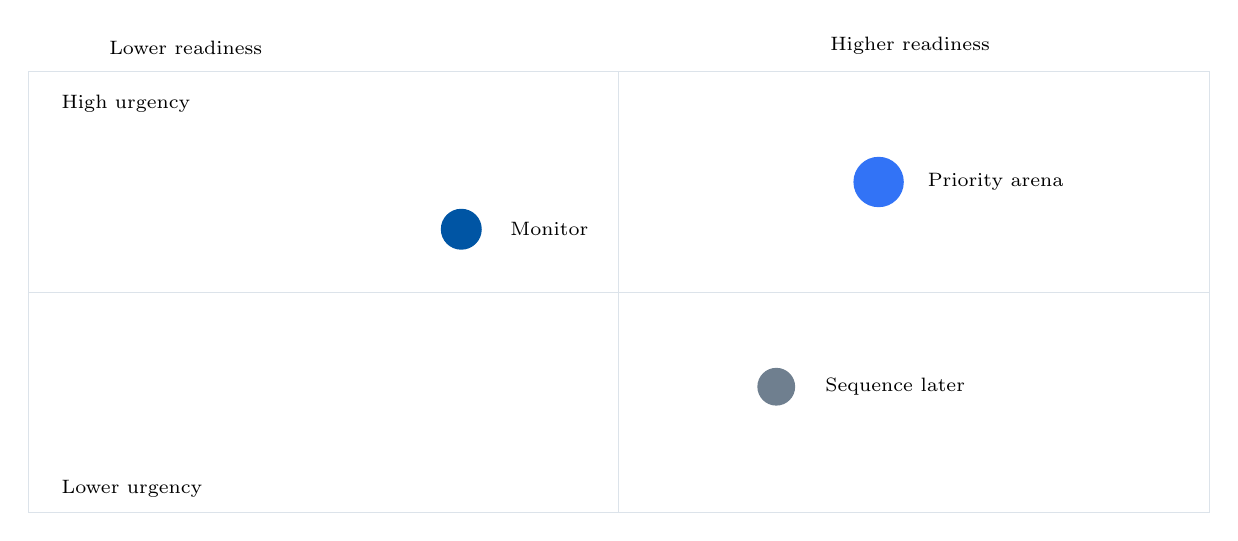
\begin{tikzpicture}[x=1mm,y=1mm]
\draw[BOLine] (0,0) rectangle (150,56);
\draw[BOLine] (75,0) -- (75,56); \draw[BOLine] (0,28) -- (150,28);
\node[anchor=west] at (3,52) {\scriptsize High urgency};
\node[anchor=west] at (3,3) {\scriptsize Lower urgency};
\node[anchor=south] at (20,57) {\scriptsize Lower readiness};
\node[anchor=south] at (112,57) {\scriptsize Higher readiness};
\fill[BOBright] (108,42) circle (3.2); \node[anchor=west] at (113,42) {\scriptsize Priority arena};
\fill[BOBlue] (55,36) circle (2.6); \node[anchor=west] at (60,36) {\scriptsize Monitor};
\fill[BOMuted] (95,16) circle (2.4); \node[anchor=west] at (100,16) {\scriptsize Sequence later};
\end{tikzpicture}
\end{center}

\clearpage
{\textcolor{BOBlue}{\scriptsize\bfseries MANAGEMENT IMPLICATIONS}}\par\vspace{-1pt}
{\Large\sffamily\bfseries\color{BONavy} Healthcare and Logistics Offer the Highest Near-Term Growth Opportunities}\par\vspace{4pt}
{\small The implication for executives is to translate the signal into a sequenced agenda: validate the facts, prioritize where the economics are strongest, and assign accountable owners for the next wave of decisions.}\par
\begin{tabularx}{\linewidth}{p{10mm}Y}
\textcolor{BOBlue}{\bfseries 1} & Prioritize management actions that change resource allocation. \\[5pt]
\textcolor{BOBlue}{\bfseries 2} & Validate the evidence base before committing capital. \\[5pt]
\textcolor{BOBlue}{\bfseries 3} & Sequence initiatives by materiality, feasibility and timing. \\[5pt]
\end{tabularx}
\vspace{6pt}

\vspace{6pt}{\textcolor{BOBlue}{\scriptsize\bfseries EXECUTION ROADMAP}}\par
\begin{center}

\begin{tikzpicture}[x=1mm,y=1mm]
\draw[very thick,BOBright] (10,18) -- (166,18);
\fill[BOBlue] (10,18) circle (2.2); \node[anchor=south,align=center,text width=34mm] at (10,22) {\scriptsize\textcolor{BOBlue}{\textbf{Now}}\\Confirm evidence};
\fill[BOBlue] (62,18) circle (2.2); \node[anchor=south,align=center,text width=34mm] at (62,22) {\scriptsize\textcolor{BOBlue}{\textbf{Next}}\\Prioritize moves};
\fill[BOBlue] (114,18) circle (2.2); \node[anchor=south,align=center,text width=34mm] at (114,22) {\scriptsize\textcolor{BOBlue}{\textbf{Then}}\\Commit resources};
\fill[BOBlue] (166,18) circle (2.2); \node[anchor=south,align=center,text width=34mm] at (166,22) {\scriptsize\textcolor{BOBlue}{\textbf{Scale}}\\Institutionalize};
\end{tikzpicture}
\end{center}

\clearpage
{\textcolor{BOBlue}{\scriptsize\bfseries CHAPTER 10}}\par\vspace{-1pt}
{\Large\sffamily\bfseries\color{BONavy} Supply Chain Concentration and Trade Tensions Pose Significant Risks to Robotics Companies}\par\vspace{4pt}
\begin{minipage}[t]{0.52\linewidth}
{\small Supply Chain Concentration and Trade Tensions Pose Significant Risks to Robotics Companies}\par
{\small The implication for executives is to translate the signal into a sequenced agenda: validate the facts, prioritize where the economics are strongest, and assign accountable owners for the next wave of decisions.}\par
\end{minipage}\hfill\begin{minipage}[t]{0.42\linewidth}

\includegraphics[width=74mm,height=54mm,keepaspectratio]{assets/image-10.png}
\end{minipage}
\vspace{5pt}
{\small The implication for executives is to translate the signal into a sequenced agenda: validate the facts, prioritize where the economics are strongest, and assign accountable owners for the next wave of decisions.}\par

\vspace{6pt}{\textcolor{BOBlue}{\scriptsize\bfseries DECISION LENS}}\par
\begin{tabularx}{\linewidth}{p{42mm}Y}
\textcolor{BOBlue}{\bfseries Question} & \textcolor{BOBlue}{\bfseries Why it matters} \\
Market direction & Separates structural change from temporary noise \\
Competitive response & Identifies where incumbents, challengers and customers may move next \\
Capital priority & Connects the argument to resource allocation and timing \\
\end{tabularx}

\clearpage
{\textcolor{BOBlue}{\scriptsize\bfseries EVIDENCE EXHIBIT}}\par\vspace{-1pt}
{\Large\sffamily\bfseries\color{BONavy} Supply Chain Concentration and Trade Tensions Pose Significant Risks to Robotics Companies}\par\vspace{4pt}

\includegraphics[width=170mm,height=88mm,keepaspectratio]{assets/chart-4.png}\vspace{5pt}
{\small The implication for executives is to translate the signal into a sequenced agenda: validate the facts, prioritize where the economics are strongest, and assign accountable owners for the next wave of decisions.}\par
{\small The exhibit should be read as directional evidence: it frames the relative magnitude, timing and management relevance of the issue rather than replacing diligence on the underlying source data.}\par

\vspace{6pt}{\textcolor{BOBlue}{\scriptsize\bfseries STRATEGIC POSITIONING MAP}}\par
\begin{center}
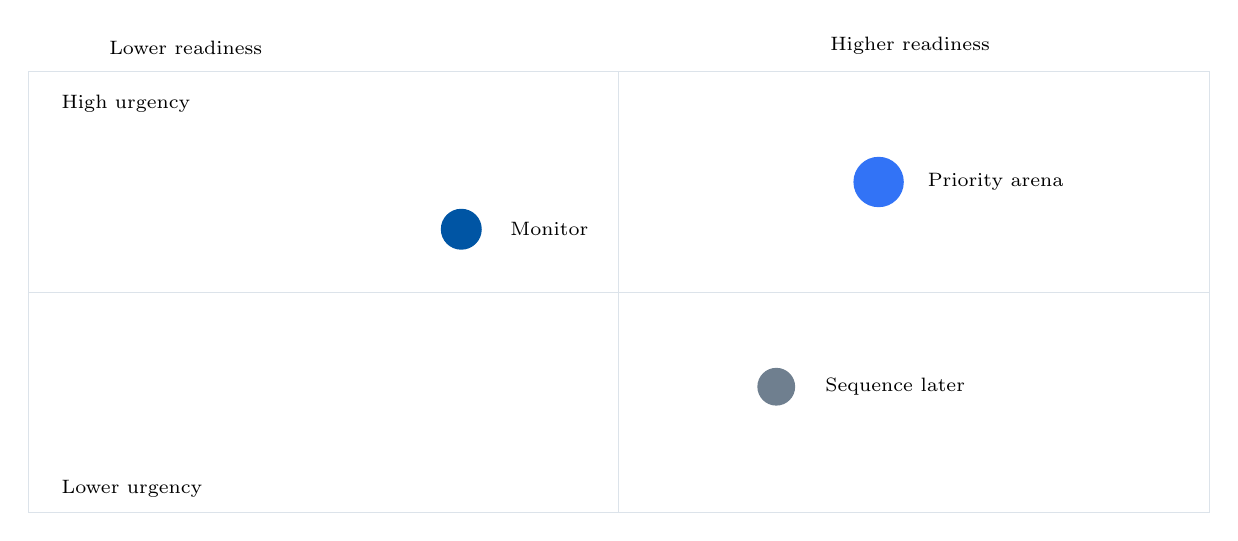
\begin{tikzpicture}[x=1mm,y=1mm]
\draw[BOLine] (0,0) rectangle (150,56);
\draw[BOLine] (75,0) -- (75,56); \draw[BOLine] (0,28) -- (150,28);
\node[anchor=west] at (3,52) {\scriptsize High urgency};
\node[anchor=west] at (3,3) {\scriptsize Lower urgency};
\node[anchor=south] at (20,57) {\scriptsize Lower readiness};
\node[anchor=south] at (112,57) {\scriptsize Higher readiness};
\fill[BOBright] (108,42) circle (3.2); \node[anchor=west] at (113,42) {\scriptsize Priority arena};
\fill[BOBlue] (55,36) circle (2.6); \node[anchor=west] at (60,36) {\scriptsize Monitor};
\fill[BOMuted] (95,16) circle (2.4); \node[anchor=west] at (100,16) {\scriptsize Sequence later};
\end{tikzpicture}
\end{center}

\clearpage
{\textcolor{BOBlue}{\scriptsize\bfseries MANAGEMENT IMPLICATIONS}}\par\vspace{-1pt}
{\Large\sffamily\bfseries\color{BONavy} Supply Chain Concentration and Trade Tensions Pose Significant Risks to Robotics Companies}\par\vspace{4pt}
{\small The implication for executives is to translate the signal into a sequenced agenda: validate the facts, prioritize where the economics are strongest, and assign accountable owners for the next wave of decisions.}\par
\begin{tabularx}{\linewidth}{p{10mm}Y}
\textcolor{BOBlue}{\bfseries 1} & Prioritize management actions that change resource allocation. \\[5pt]
\textcolor{BOBlue}{\bfseries 2} & Validate the evidence base before committing capital. \\[5pt]
\textcolor{BOBlue}{\bfseries 3} & Sequence initiatives by materiality, feasibility and timing. \\[5pt]
\end{tabularx}
\vspace{6pt}

\vspace{6pt}{\textcolor{BOBlue}{\scriptsize\bfseries EXECUTION ROADMAP}}\par
\begin{center}

\begin{tikzpicture}[x=1mm,y=1mm]
\draw[very thick,BOBright] (10,18) -- (166,18);
\fill[BOBlue] (10,18) circle (2.2); \node[anchor=south,align=center,text width=34mm] at (10,22) {\scriptsize\textcolor{BOBlue}{\textbf{Now}}\\Confirm evidence};
\fill[BOBlue] (62,18) circle (2.2); \node[anchor=south,align=center,text width=34mm] at (62,22) {\scriptsize\textcolor{BOBlue}{\textbf{Next}}\\Prioritize moves};
\fill[BOBlue] (114,18) circle (2.2); \node[anchor=south,align=center,text width=34mm] at (114,22) {\scriptsize\textcolor{BOBlue}{\textbf{Then}}\\Commit resources};
\fill[BOBlue] (166,18) circle (2.2); \node[anchor=south,align=center,text width=34mm] at (166,22) {\scriptsize\textcolor{BOBlue}{\textbf{Scale}}\\Institutionalize};
\end{tikzpicture}
\end{center}

\clearpage
{\textcolor{BOBlue}{\scriptsize\bfseries DISCLAIMER}}\par\vspace{-1pt}
{\Large\sffamily\bfseries\color{BONavy} This report is a management consulting analysis, not investment advice}\par\vspace{4pt}
\vspace{2pt}{\color{BOBright}\rule{\linewidth}{1pt}}\vspace{5pt}
{\small This document has been prepared by BlueOcean for strategy discussion, industry analysis and executive decision support. It is not intended to constitute investment advice, securities research, legal advice, tax advice, audit assurance, or a recommendation to buy or sell any security or financial instrument. The analysis relies on public sources, model-assisted synthesis and management-consulting judgment. Market estimates, forecasts and scenarios are directional and should be independently validated before they are used for investment, financing, transaction, regulatory or operational decisions.}\par
\vspace{6pt}{\small\color{BOMuted} BlueOcean does not guarantee the completeness or accuracy of third-party information and accepts no responsibility for decisions made solely on the basis of this document.}

\end{document}
